\documentclass[10pt, oneside]{article} 
\usepackage{amsmath, amsthm, amssymb, calrsfs, wasysym, verbatim, bbm, color, graphics, geometry, esint}
\usepackage{float}


\geometry{tmargin=.75in, bmargin=.75in, lmargin=.75in, rmargin = .75in}  

\newcommand{\bbR}{\mathbb{R}}
\newcommand{\bbC}{\mathbb{C}}
\newcommand{\bbZ}{\mathbb{Z}}
\newcommand{\bbN}{\mathbb{N}}
\newcommand{\bbQ}{\mathbb{Q}}
\newcommand{\Cdot}{\boldsymbol{\cdot}}
\newcommand{\scA}{\mathscr{A}}
\newcommand{\curl}{\text{curl}}

\theoremstyle{definition}
\newtheorem{exmp}{Example}[section]
\newtheorem{thm}{Theorem}
\newtheorem{defn}{Definition}
\newtheorem{prop}{Proposition}
\newtheorem{conv}{Convention}
\newtheorem{rem}{Remark}
\newtheorem{lem}{Lemma}
\newtheorem{cor}{Corollary}
% Copyright 2021 Paolo Adajar (padajar.com, paoloadajar@mit.edu)
% 
% Permission is hereby granted, free of charge, to any person obtaining a copy of this software and associated documentation files (the "Software"), to deal in the Software without restriction, including without limitation the rights to use, copy, modify, merge, publish, distribute, sublicense, and/or sell copies of the Software, and to permit persons to whom the Software is furnished to do so, subject to the following conditions:
%
% The above copyright notice and this permission notice shall be included in all copies or substantial portions of the Software.
% 
% THE SOFTWARE IS PROVIDED "AS IS", WITHOUT WARRANTY OF ANY KIND, EXPRESS OR IMPLIED, INCLUDING BUT NOT LIMITED TO THE WARRANTIES OF MERCHANTABILITY, FITNESS FOR A PARTICULAR PURPOSE AND NONINFRINGEMENT. IN NO EVENT SHALL THE AUTHORS OR COPYRIGHT HOLDERS BE LIABLE FOR ANY CLAIM, DAMAGES OR OTHER LIABILITY, WHETHER IN AN ACTION OF CONTRACT, TORT OR OTHERWISE, ARISING FROM, OUT OF OR IN CONNECTION WITH THE SOFTWARE OR THE USE OR OTHER DEALINGS IN THE SOFTWARE.

\usepackage{fullpage}
\usepackage{enumitem}
\usepackage{amsfonts, amssymb, amsmath,amsthm}
\usepackage{mathtools}
\usepackage[pdftex, pdfauthor={\name}, pdftitle={\classnum~\assignment}]{hyperref}
\usepackage[dvipsnames]{xcolor}
\usepackage{bbm}
\usepackage{graphicx}
\usepackage{mathrsfs}
\usepackage{pdfpages}
\usepackage{tabularx}
\usepackage{pdflscape}
\usepackage{makecell}
\usepackage{booktabs}
\usepackage{natbib}
\usepackage{caption}
\usepackage{subcaption}
\usepackage{physics}
\usepackage[many]{tcolorbox}
\usepackage{version}
\usepackage{ifthen}
\usepackage{cancel}
\usepackage{listings}
\usepackage{courier}

\usepackage{tikz}
\usepackage{istgame}

\hypersetup{
	colorlinks=true,
	linkcolor=blue,
	filecolor=magenta,
	urlcolor=blue,
}

\setlength{\parindent}{0mm}
\setlength{\parskip}{2mm}

\setlist[enumerate]{label=({\alph*})}
\setlist[enumerate, 2]{label=({\roman*})}

\allowdisplaybreaks[1]

\newcommand{\psetheader}{
	\ifthenelse{\isundefined{\collaborators}}{
		\begin{center}
			{\setlength{\parindent}{0cm} \setlength{\parskip}{0mm}
				
				{\textbf{\classnum~\semester:~\assignment} \hfill \name}
				
				\subject \hfill \href{mailto:\email}{\tt \email}
				
				Instructor(s):~\instructors \hfill Due Date:~\duedate	
				
				\hrulefill}
		\end{center}
	}{
		\begin{center}
			{\setlength{\parindent}{0cm} \setlength{\parskip}{0mm}
				
				{\textbf{\classnum~\semester:~\assignment} \hfill \name\footnote{Collaborator(s): \collaborators}}
				
				\subject \hfill \href{mailto:\email}{\tt \email}
				
				Instructor(s):~\instructors \hfill Due Date:~\duedate	
				
				\hrulefill}
		\end{center}
	}
}

\renewcommand{\thepage}{\classnum~\assignment \hfill \arabic{page}}

\makeatletter
\def\points{\@ifnextchar[{\@with}{\@without}}
\def\@with[#1]#2{{\ifthenelse{\equal{#2}{1}}{{[1 point, #1]}}{{[#2 points, #1]}}}}
\def\@without#1{\ifthenelse{\equal{#1}{1}}{{[1 point]}}{{[#1 points]}}}
\makeatother

\newtheoremstyle{theorem-custom}%
{}{}%
{}{}%
{\itshape}{.}%
{ }%
{\thmname{#1}\thmnumber{ #2}\thmnote{ (#3)}}

\theoremstyle{theorem-custom}

\newtheorem{theorem}{Theorem}
\newtheorem{lemma}[theorem]{Lemma}
\newtheorem{example}[theorem]{Example}

\newenvironment{problem}[1]{\color{black} #1}{}

\newenvironment{solution}{%
	\leavevmode\begin{tcolorbox}[breakable, colback=green!5!white,colframe=green!75!black, enhanced jigsaw] \proof[\scshape Solution:] \setlength{\parskip}{2mm}%
	}{\renewcommand{\qedsymbol}{$\blacksquare$} \endproof \end{tcolorbox}}

\newenvironment{reflection}{\begin{tcolorbox}[breakable, colback=black!8!white,colframe=black!60!white, enhanced jigsaw, parbox = false]\textsc{Reflections:}}{\end{tcolorbox}}

\newcommand{\qedh}{\renewcommand{\qedsymbol}{$\blacksquare$}\qedhere}

\definecolor{mygreen}{rgb}{0,0.6,0}
\definecolor{mygray}{rgb}{0.5,0.5,0.5}
\definecolor{mymauve}{rgb}{0.58,0,0.82}

% from https://github.com/satejsoman/stata-lstlisting
% language definition
\lstdefinelanguage{Stata}{
	% System commands
	morekeywords=[1]{regress, reg, summarize, sum, display, di, generate, gen, bysort, use, import, delimited, predict, quietly, probit, margins, test},
	% Reserved words
	morekeywords=[2]{aggregate, array, boolean, break, byte, case, catch, class, colvector, complex, const, continue, default, delegate, delete, do, double, else, eltypedef, end, enum, explicit, export, external, float, for, friend, function, global, goto, if, inline, int, local, long, mata, matrix, namespace, new, numeric, NULL, operator, orgtypedef, pointer, polymorphic, pragma, private, protected, public, quad, real, return, rowvector, scalar, short, signed, static, strL, string, struct, super, switch, template, this, throw, transmorphic, try, typedef, typename, union, unsigned, using, vector, version, virtual, void, volatile, while,},
	% Keywords
	morekeywords=[3]{forvalues, foreach, set},
	% Date and time functions
	morekeywords=[4]{bofd, Cdhms, Chms, Clock, clock, Cmdyhms, Cofc, cofC, Cofd, cofd, daily, date, day, dhms, dofb, dofC, dofc, dofh, dofm, dofq, dofw, dofy, dow, doy, halfyear, halfyearly, hh, hhC, hms, hofd, hours, mdy, mdyhms, minutes, mm, mmC, mofd, month, monthly, msofhours, msofminutes, msofseconds, qofd, quarter, quarterly, seconds, ss, ssC, tC, tc, td, th, tm, tq, tw, week, weekly, wofd, year, yearly, yh, ym, yofd, yq, yw,},
	% Mathematical functions
	morekeywords=[5]{abs, ceil, cloglog, comb, digamma, exp, expm1, floor, int, invcloglog, invlogit, ln, ln1m, ln, ln1p, ln, lnfactorial, lngamma, log, log10, log1m, log1p, logit, max, min, mod, reldif, round, sign, sqrt, sum, trigamma, trunc,},
	% Matrix functions
	morekeywords=[6]{cholesky, coleqnumb, colnfreeparms, colnumb, colsof, corr, det, diag, diag0cnt, el, get, hadamard, I, inv, invsym, issymmetric, J, matmissing, matuniform, mreldif, nullmat, roweqnumb, rownfreeparms, rownumb, rowsof, sweep, trace, vec, vecdiag, },
	% Programming functions
	morekeywords=[7]{autocode, byteorder, c, _caller, chop, abs, clip, cond, e, fileexists, fileread, filereaderror, filewrite, float, fmtwidth, has_eprop, inlist, inrange, irecode, matrix, maxbyte, maxdouble, maxfloat, maxint, maxlong, mi, minbyte, mindouble, minfloat, minint, minlong, missing, r, recode, replay, return, s, scalar, smallestdouble,},
	% Random-number functions
	morekeywords=[8]{rbeta, rbinomial, rcauchy, rchi2, rexponential, rgamma, rhypergeometric, rigaussian, rlaplace, rlogistic, rnbinomial, rnormal, rpoisson, rt, runiform, runiformint, rweibull, rweibullph,},
	% Selecting time-span functions
	morekeywords=[9]{tin, twithin,},
	% Statistical functions
	morekeywords=[10]{betaden, binomial, binomialp, binomialtail, binormal, cauchy, cauchyden, cauchytail, chi2, chi2den, chi2tail, dgammapda, dgammapdada, dgammapdadx, dgammapdx, dgammapdxdx, dunnettprob, exponential, exponentialden, exponentialtail, F, Fden, Ftail, gammaden, gammap, gammaptail, hypergeometric, hypergeometricp, ibeta, ibetatail, igaussian, igaussianden, igaussiantail, invbinomial, invbinomialtail, invcauchy, invcauchytail, invchi2, invchi2tail, invdunnettprob, invexponential, invexponentialtail, invF, invFtail, invgammap, invgammaptail, invibeta, invibetatail, invigaussian, invigaussiantail, invlaplace, invlaplacetail, invlogistic, invlogistictail, invnbinomial, invnbinomialtail, invnchi2, invnF, invnFtail, invnibeta, invnormal, invnt, invnttail, invpoisson, invpoissontail, invt, invttail, invtukeyprob, invweibull, invweibullph, invweibullphtail, invweibulltail, laplace, laplaceden, laplacetail, lncauchyden, lnigammaden, lnigaussianden, lniwishartden, lnlaplaceden, lnmvnormalden, lnnormal, lnnormalden, lnwishartden, logistic, logisticden, logistictail, nbetaden, nbinomial, nbinomialp, nbinomialtail, nchi2, nchi2den, nchi2tail, nF, nFden, nFtail, nibeta, normal, normalden, npnchi2, npnF, npnt, nt, ntden, nttail, poisson, poissonp, poissontail, t, tden, ttail, tukeyprob, weibull, weibullden, weibullph, weibullphden, weibullphtail, weibulltail,},
	% String functions 
	morekeywords=[11]{abbrev, char, collatorlocale, collatorversion, indexnot, plural, plural, real, regexm, regexr, regexs, soundex, soundex_nara, strcat, strdup, string, strofreal, string, strofreal, stritrim, strlen, strlower, strltrim, strmatch, strofreal, strofreal, strpos, strproper, strreverse, strrpos, strrtrim, strtoname, strtrim, strupper, subinstr, subinword, substr, tobytes, uchar, udstrlen, udsubstr, uisdigit, uisletter, ustrcompare, ustrcompareex, ustrfix, ustrfrom, ustrinvalidcnt, ustrleft, ustrlen, ustrlower, ustrltrim, ustrnormalize, ustrpos, ustrregexm, ustrregexra, ustrregexrf, ustrregexs, ustrreverse, ustrright, ustrrpos, ustrrtrim, ustrsortkey, ustrsortkeyex, ustrtitle, ustrto, ustrtohex, ustrtoname, ustrtrim, ustrunescape, ustrupper, ustrword, ustrwordcount, usubinstr, usubstr, word, wordbreaklocale, worcount,},
	% Trig functions
	morekeywords=[12]{acos, acosh, asin, asinh, atan, atanh, cos, cosh, sin, sinh, tan, tanh,},
	morecomment=[l]{//},
	% morecomment=[l]{*},  // `*` maybe used as multiply operator. So use `//` as line comment.
	morecomment=[s]{/*}{*/},
	% The following is used by macros, like `lags'.
	morestring=[b]{`}{'},
	% morestring=[d]{'},
	morestring=[b]",
	morestring=[d]",
	% morestring=[d]{\\`},
	% morestring=[b]{'},
	sensitive=true,
}

\lstset{ 
	backgroundcolor=\color{white},   % choose the background color; you must add \usepackage{color} or \usepackage{xcolor}; should come as last argument
	basicstyle=\footnotesize\ttfamily,        % the size of the fonts that are used for the code
	breakatwhitespace=false,         % sets if automatic breaks should only happen at whitespace
	breaklines=true,                 % sets automatic line breaking
	captionpos=b,                    % sets the caption-position to bottom
	commentstyle=\color{mygreen},    % comment style
	deletekeywords={...},            % if you want to delete keywords from the given language
	escapeinside={\%*}{*)},          % if you want to add LaTeX within your code
	extendedchars=true,              % lets you use non-ASCII characters; for 8-bits encodings only, does not work with UTF-8
	firstnumber=0,                % start line enumeration with line 1000
	frame=single,	                   % adds a frame around the code
	keepspaces=true,                 % keeps spaces in text, useful for keeping indentation of code (possibly needs columns=flexible)
	keywordstyle=\color{blue},       % keyword style
	language=Octave,                 % the language of the code
	morekeywords={*,...},            % if you want to add more keywords to the set
	numbers=left,                    % where to put the line-numbers; possible values are (none, left, right)
	numbersep=5pt,                   % how far the line-numbers are from the code
	numberstyle=\tiny\color{mygray}, % the style that is used for the line-numbers
	rulecolor=\color{black},         % if not set, the frame-color may be changed on line-breaks within not-black text (e.g. comments (green here))
	showspaces=false,                % show spaces everywhere adding particular underscores; it overrides 'showstringspaces'
	showstringspaces=false,          % underline spaces within strings only
	showtabs=false,                  % show tabs within strings adding particular underscores
	stepnumber=2,                    % the step between two line-numbers. If it's 1, each line will be numbered
	stringstyle=\color{mymauve},     % string literal style
	tabsize=2,	                   % sets default tabsize to 2 spaces
%	title=\lstname,                   % show the filename of files included with \lstinputlisting; also try caption instead of title
	xleftmargin=0.25cm
}



\title{UChicago Point Set Topology}
\author{Notes by Agustín Esteva, Lectures by Calegari, Books by , }
\date{Academic Year 2024-2025}

\begin{document}

\maketitle
\tableofcontents

\vspace{.25in}

\section{Lectures}

\subsection{Tuesday, Jan 21: Continuous Functions and Homeomorphisms}
\begin{defn}
    We say $X$ and $Y$ are \textbf{homeomorphic} if there exits some $f: X \to Y$ and $g: Y \to X$ which are both continuous such that $f\circ g: Y\to Y$ is identity on $Y$ and $g\circ f: X \to X$ is the identity on $X.$

    We say that $f$ and $g$ are \textbf{homeomorphisms}.
\end{defn}

\begin{defn}
    Suppose $f: X\to Y$ is injective, then we say $f$ is an \textbf{embedding} if $f$ unto its image is a homeomorphism.
\end{defn}
\begin{rem}
    To give a non-example, we let $X = [0,2\pi)$ and $Y = \bbR^2,$ and we define 
    $f; X\to Y$ by sending $X$ to the unit circle: 
    \begin{figure}[H]
        \centering
        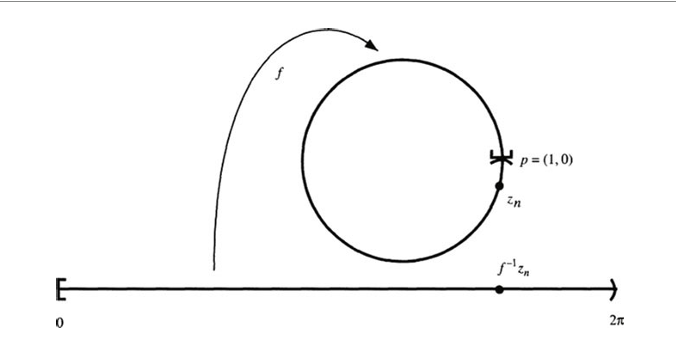
\includegraphics[width=0.5\linewidth]{Images/Pughnonexample.png}
    \end{figure}
\end{rem}
\begin{thm}
    We assert that:
    \begin{enumerate}
        \item Constant functions are continuous.
        \item If $A \subset X$ and $i$ is the inclusion of $A$ as a subset of $X.$ That is, $i$ is an injective map from $A \to X,$ then $i$ continuous. 
        \item Suppose $f: X\to Y$ and $g: Y\to Z,$ then if $f$ and $g$ are continuous, then $f \circ g$ is continuous.
        \item Suppose $A\subset X$ and $f: X\to Y$ is continuous, then $f|_A: A \to Y$ is continuous.
        \item Suppose $f: X\to Y,$ where $Y\subset Z,$ then if $f$ is continuous, then $\hat{f}: X\to Z$ is continuous.
        \item Suppose $X= \bigcup U_\alpha,$ where $U_\alpha$ is open for each $\alpha.$ If $f: X\to Y$ such that $f|_{U_\alpha}: U_\alpha \to Y$ is continuous for each $\alpha,$ then $f$ is continuous.
        \item Suppose $X = A \cup B,$ where $A,B$ are closed. Suppose we have  $f: X\to Y$ such that $f|_A$ and $f|_B$ are both continuous, then $f$ is continuous.
        \item We say $f: Y \to \prod X_\alpha$ is continuous if and only if the ``coordinate functions," $f_\alpha = \prod_\alpha f$ is continuous for all $\alpha.$
    \end{enumerate}
\end{thm}
\begin{proof}
    We give a proof for (f): Let $U$ be an open set in $Y.$ By continuity of each $f$ restriction, we have that $f^{-1}|_{U_\alpha}(U)$ is open in $U_\alpha.$
    Notice that $f^{-1}|_{U_\alpha}(U) = f^{-1}(U) \cap U_\alpha,$ which is open in both $U_\alpha$ and in $X$ (since the intersection of open is open). Moreover, we have that 
    \[f^{-1}(U) = \bigcup(f^{-1}(U) \cap U_\alpha),\] which is open in $X.$

    Proof of (g): Suppose $K\subset Y$ is closed, then $f^{-1}|_A(K)$ is closed in $A$ and thus closed in $X,$ similarly for $B.$ Then 
    \[f^{-1}(K) = f^{-1}|_A(K) \cup f^{-1}|_B (K)\] is closed.
\end{proof}
\begin{rem}
    Note that (f) is not true if we replace $U_\alpha$ for closed sets. To see this, take $X = \bigcup K_\alpha,$ where $K_\alpha$ is each point in $X.$ Then there are a lot of examples.
\end{rem}
\begin{defn}
    Suppose $X$ is a set and $(Y,d)$ is a metric space. We say a sequence of functions $\{f_n : X\to Y\}$ converges uniformly to $f: X\to Y$ if for all $\epsilon>0,$ there exists an $N\in \bbN$ such that  if $n\geq N,$ we have that 
    \[d(f_n(x) - f(x))< \epsilon, \quad \forall x\in X \iff ||f - f_n|| < \epsilon.\]
\end{defn}
\begin{thm}
    Let $f_n: X\to Y$ be continuous, where $X$ is a set and $(Y,d)$ is a metric space. If $f_n \to f$ uniformly, then $f$ is continuous.
\end{thm}
\begin{proof}
    Let $V\subset Y$ be open. Let $x\in f^{-1}(V).$ We want to find some open $U\subset f^{-1}(V)$ such that $x\in U.$ That is, $f(U)\subset V.$ Let $f(x) = y.$  Since $V$ is open, then there exists an $\epsilon>0$ such that $B_\epsilon(y)\subset V.$ Now we want to find an open neighborhood of $x$ such that its image is contained in this ball. By uniform convergence, there exists an $N$ such that if $n\geq N,$ we have that $d(f_n(x), f(x))< \frac{\epsilon}{3}$ for all $x\in X.$ Since $f_N$ is continuous, then there exists a $x\in U$ such that $f_N(U)\subset B_\frac{\epsilon}{3}(f_N(x)).$ Thus, for all $y\in U:$
    \[d(f(y), f_N(y))< \frac{\epsilon}{3}, \quad d(f_N(y), f_N(x)) < \frac{\epsilon}{3}, \quad d(f_N(x), f(x))< \frac{\epsilon}{3}.\]
\end{proof}

\newpage
\subsection{Thursday, Jan 23: Connectedness}
\begin{defn}
    A \textbf{separation} of a topological space $X$ is a decomposition 
    \[X = A \sqcup B\] such that $A,B$ are both open and nonempty.
\end{defn}
\begin{defn}
    A topological space $X$ is \textbf{connected} if it does not admit a separation.
\end{defn}
\begin{lemma}
    $X$ is connected if and only if, whenever we write $X = A \sqcup B,$ where $A$ and $B$ are nonempty, then either $A \cap B' \neq \emptyset$ or $A' \cap B \neq \emptyset.$
\end{lemma}
\begin{proof}
    Suppose $X$ is connected, then without loss of generality, $A$ is not closed. Thus, \[A' \not \subset A \implies A' \cap B \neq \emptyset.\] If, on the other hand, $X$ is disconnected, then $A$ and $B$ are both closed, and thus \[A' \cap B = A \cap B' = A \cap B = \emptyset.\]
\end{proof}
\begin{lemma}
    Suppose $X = C\sqcup D,$ where $C,D$ are both open. Suppose that $Y\subset X$ is connected in the subspace topoogy, then either $Y\subset C$ or $Y\subset D.$
\end{lemma}
\begin{proof}
    Consider that 
    \[Y = Y\cap C \sqcup Y\cap D,\] where both of the terms in the right are open in $Y$ because both $C$ and $D$ are open. Thus, by connectedness of $Y,$ at least one of these must be empty.
\end{proof}
\begin{thm}
    Suppose $X = \bigcup_\alpha X_\alpha,$ where every $X_\alpha$ is connected and there exists some $p \in \bigcap X_\alpha,$ then $X$ is connected.
\end{thm}
\begin{proof}
    Suppose $X = A\sqcup B,$ both open. By Lemma 2, we have that for all $\alpha,$ we have that either $X_\alpha \subset A$ or $X_\alpha \subset B.$ Without loss of generality, $p \in A,$ and thus $X_\alpha \subset A$ for all $\alpha,$ and thus $B$ is empty.
\end{proof}

\begin{thm}
    Suppose $A \subset X,$ where $A$ is connected. If $A\subset B \subset \overline{A},$ then $B$ is connected.
\end{thm}
\begin{proof}
    Suppose $B = C \sqcup D,$ where $C,D$ open and nonempty. Since $A$ is connected, then by lemma 2, without loss of generality, we can say that $A\subset C.$ Thus, $\overline{A}\subset \overline{C} = C,$ which is disjoint from $D,$ and thus 
    \[B \cap D = \emptyset.\]
\end{proof}
\begin{thm}
    Suppose $X$ is connected and $f: X\to Y$ is continuous. Then $f(X)$ is connected.
\end{thm}
\begin{proof}
    Let $f(X) = A\sqcup B,$ $A,B$ nonempty and open. Since $f$ is continuous, then $X = f^{-1}(A)\sqcup f^{-1}(B),$ where they are both open by continuity and nonempty by surjectivity.  
\end{proof}

\begin{thm}
    Suppose $X$ and $Y$ are connected, then $X \times Y$ is connected.
\end{thm}
\begin{proof}
    Let $x\in X.$ We claim that $\{x\}\times Y$ is homeomorphic to $Y.$ The homeomorphism is $\pi,$ the projection map. Thus, $A_x = \{x\}\times Y$ is connected. Similarly, $B_x = X \times \{y\}$ is connected for every $y \in Y.$ Thus, since $T_{x,y} = A_x \cap B_x = (x,y),$ then by Theorem 3, we have that 
    \[X = \bigcup_{y \in Y} T_{x,y}\] is connected.
\end{proof}
We can obviously extend this to a finite product of connected spaces. What about for infinite products?

\begin{defn}
    Let $X_\alpha$ be a collection of spaces. We say that the \textbf{box topology} on $\prod X_\alpha$ is the topology separated by the basis 
    \[B  = \{\prod U_\alpha, \; : \; U_\alpha \subset X_\alpha \; \text{is open}\}.\].
\end{defn}
\begin{exmp}
    $\bbR^N$ is connected in the product topology but not connected in the box topology. To see this, think of $\bbR^ = \{(x_1, x_2, \dots) \; : \; x_i \in \bbR\}$ and think of $\bbR^N = \text{bounded sequences} \sqcup \text{unbounded sequences}.$ We claim that these are both open in the box topology: Let $a \in \text{bounded sequence}.$ Thus, there exists some $C$ such that for all $a_i,$ $a_i \leq C.$ Consider 
    \[U_i = (x_1 - 1, x_1 + 1)\times (x_2 - 1, x_2 + 1)\times \cdots,\] which is an open set, and is a basis element in the box topology since every point in $U_i$ is bounded by $C + 1.$ An identical argument proves that $\{\text{unbounded sequences}\}$ are unbounded. Thus, $\bbR^N$ is not connected in the box topology. 
\end{exmp}

\begin{thm}
    Suppose $X_\alpha$ is any collection of connected spaces, then $\prod X_\alpha$ is connected in the product topology.
\end{thm}
\begin{proof}
    It suffices to find a connected $K \subset X$ such that for every open $U \subset X,$ we have that $K \cap U \neq \emptyset.$ To find this, we will use Theorem 3. let $x\in X,$ where $x = (x_\alpha)_\alpha.$ Let $I$ be a finite set of indices, and define \[K_i := \{y \; : \; y_\alpha = x_\alpha, \quad \alpha \notin I\}.\] We remark that $K_I$ is homeomorphic to $\prod_{\alpha \in I} X_\alpha$ under the projection homeomorphism. $\prod_{I}X_\alpha$ is connected by Theorem 3, and thus $K_I$ is connected and contains $x.$ 
    \[K = \bigcup_{\text{all finite $I$ index sets}}K_I\] is connected again by Theorem 3. For any nonempty open basis in the product topology $U\subset X,$ we claim that $K\cap U \neq \emptyset.$ To see this, let $U = \prod U_\allowdisplaybreaks,$ where $U_\alpha = X_\alpha$ except for finitely many indices ($I$). Since each $U_\alpha$ is nonempty, then for $\alpha \in I,$ we choose some $u_\alpha \in U_\alpha.$ And for $\alpha \notin I,$ then choose $u_\alpha = x_\alpha.$ It is not hard to see that $u_\alpha \in K$ and that $u_\alpha \in U.$ Thus, $X$ is connected.
\end{proof}
\newpage

\subsection{Tuesday, Jan 28: Compactness}
\begin{defn}
    Let $X$ be a space, and let $x,y \in X.$ A \textbf{path} in $X$ is defined to be the continuous map $f: [0,1] \to X$ such that
    \[f(0) = x, \qquad f(1) = y.\]
\end{defn}

\begin{defn}
    A space $X$ is \textbf{path connected} if for any $x, y \in X,$ there is a path in $X$ from $x$ to $y.$
\end{defn}

\begin{prop}
    If $X$ is path connected, then $X$ is connected.
\end{prop}
\begin{proof}
    Consider that $f([0,1])\subset X$ is a connected subspace of $X$ by the continuity of $f.$ Let $x \in X.$ For any $y\in Y,$ choose the path $f_y$ such that $f_y(0) = x$ and $f_y(1)= y.$ Let $P_y:= f_y([0,1])\subset X.$ Since $y\in P_y$ for all $y,$ then $X = \bigcup_y P_y,$ and since $x\in P_y$ for all $y,$ then $X$ is connected.
\end{proof}
\begin{rem}
    The converse fails, see 
    \[X = \sin(\frac{1}{x}) \cup [0,1]\]
\end{rem}

\begin{thm}
    (IVT) Let $X$ be connected and let $f: X\to \bbR$ be continuous. If $a,b \in X$ and there exists some $c\in [f(a), f(b)],$ then there exists some $\gamma \in [a,b]$ such that $f(\gamma) = c.$
\end{thm}
\begin{proof}
    Suppose not, then $c \notin f(X),$ then $f(X)\subset [-\infty, c) \cup (c, \infty].$ Both of these sets are open, and thus the inverses are open and disjoint. Neither is empty and we get that their union is all of $X.$ Thus, $X$ is not connected, which is a contradiction.
\end{proof}

\begin{defn}
    We say that $X$ is \textbf{compact} if any open cover has a finite open subcover.
\end{defn}
\begin{exmp}
We give some examples.
    \begin{enumerate}
        \item $\bbR$ is not compact. Let $\{(-n, n)\}_{n\in \bbN}$ be the open cover of $\bbR.$ Obviously there is no finite subcover (say, of cardinality $N$), since then there would exist some $(-N, N)$ that does not contain $N \in \bbR.$
        \item $(0,1)$ is not compact since it is homeomorphic to $\bbR.$
        \item $[0,1]$ is compact. To see this, let $\{U_\alpha\}$ be a cover of $X.$ Thus, $0 \in U_\alpha$ for some $\alpha,$ and thus there exists some $p>0$ such that $B_p(0) = [0,p)\subset U_\alpha$ for some $\alpha.$ Since $p\in X,$ then $p\in U_\beta,$ and thus there exists some $q>p$ such that $[0,q]\subset U_\alpha \cup U_\beta.$ Define 
        \[p = \sup\{q \; \: [0,q) \subset \text{finite subcover}\},\] we claim that $p = 1.$ Suppose that $p<1,$ then $p\in [0,1]$ and so $p\in U_\beta$ for some $\beta.$ By definition, there must exist some $q$ such that $[0,q]\subset \{U_i\}.$ But then we see that since $p\in U_\beta,$ and $U_\beta$ is open, then $(p-\epsilon, p+\epsilon)\subset U_\beta,$ but then $\{U_i\} \cup U_\beta \supset [0, p + \frac{\epsilon}{2}] \ni q,$ which is a contradiction to the size of $p.$  
    \end{enumerate}
\end{exmp}

\begin{rem}
    To see that $X$ is compact, it suffices to show that every open cover of $X$ by basis elements has a finite subcover.
\end{rem}

\begin{thm}
    If $X$ is compact and $Y\subset X$ is closed, then $Y$ is compact.
\end{thm}
\begin{proof}
    Let $\{U_\alpha\}$ be an open cover of $Y.$ Then we have that for every $\alpha,$ there exist some open $V_\alpha \in X$ such that $V_\alpha \cap Y = U_\alpha.$ Then we have that $Y \subset V_\alpha.$ Moreover, since $Y$ is closed, then $X\setminusm Y$ is open in $X,$ and so 
    \[\bigcup V_\alpha \cup (X\setminusm Y) \supset X.\] By the compactness of $X,$ we have a finite subset $\{V_{\alpha_i}\}\cup (X\setminus Y) \supset X,$ and thus intersecting with $Y$ gives an open finite subcover of $X.$
\end{proof}

\begin{thm}
    Suppose $f$ is Hausdorff. If $Y\subset X$ is compact, then $Y$ is closed.
\end{thm}
\begin{proof}
    It suffices to show that for every $x\in X\setminus Y,$ there exists some $r>0$ such that $B_r(x) \cap Y = \emptyset.$ Fix $x\in X \setminus Y.$ Since $X$ is Hausdorff, then for all $y\in Y,$ there exists a set $V_y\ni y$ and $W_y \ni x$ such that $V_y \cap W_y = \emptyset.$ Clearly, $\{V_y\}$ is an open cover, and thus let $\{V_{y_i}\}$ be the open finite subcover. Moreover, we have that 
    \[\bigcup V_{y_i} \cap \bigcap W_{y_i} = \emptyset.\] Since $x\in W_{y_i}$ for all $x,$ and each is open, then the finite intersection is open. Thus, we have that $Y \cap \bigcap W_{y_i} = \emptyset$ and $\bigcap W_{y_i} \ni x.$
\end{proof}
\begin{cor}
    If $X$ is compact and Hausdorff and $Y\subset X$ is closed, then $Y$ is compact. Moreover, for any $x\in X\setminus Y,$ there exist open $V \supset Y$ and $x\in U$ such that $V\cap U = \emptyset.$
\end{cor}
This corollary separates a closed set from a point, and we say $X$ is \textbf{regular}. We say $X$ is \textbf{normal} if it separates from closed sets in $Y \setminus X.$

\begin{thm}
    Suppose $f: X\to Y$ be continuous with $X$ compact. Then $f(X)$ is compact.
\end{thm}
\begin{proof}
    Let $\{U_\alpha\}$ be an open cover of $f(X).$ Then $\{f^{-1}(U_\alpha)\}$ is an open cover of $X,$ and thus $\{f^{-1}(U_{\alpha_i})\}$ is a finite open cover with 
    \[X \subset \bigcup_{i=1}^n f^{-1}(U_{\alpha_i}) \implies f(X) \subset \bigcup_{i=1}^n U_{\alpha_i}.\]
\end{proof}
\begin{thm}
    Suppose $f: X\to Y$ is a continuous bijection with $X$ compact and $Y$ Hausdorff. Then $f$ is a homeomorphism.
\end{thm}
\begin{proof}
    We have that $f^{-1}$ is continuous if and only if $f(F)$ is closed ($F$ closed). Let $K\subset X$ be closed, then $K$ is compact, and thus $f(K)$ is compact, and thus since $Y$ is closed, then $f(K)$ is closed. 
\end{proof}

\newpage
\subsection{Tuesday, Feb 4: Applications of Tychonoff's Theorem}
\begin{exmp}
    Suppose $X$ is equipped with the discrete topology. Then if we say that 
    \[\beta X = \overline{F(X)}\subset \prod \text{Compact spaces with upper bound on card. and exist continuous function from X}.\] Then 
    \[\beta X = \text{ultrafilters on X}.\] For all $A\subset X, U_A\subset \beta X,$ where 
    \[U_A := \{\mathcal{F}\; ; \; A\subset \mathcal{F}\}.\] We claim that $\{U_A\}$ is a basis for a topology. 
    \[X\to \beta X\]
    \[x \to \{\mathcal{F_x} \; \text{principal ultrafilter gen by $x$}\}\]
\end{exmp}
\begin{prop}
    \begin{enumerate}
        \item This map is homeomorphic
        \item $\beta X$ is compact and Hausdorff
    \end{enumerate}
\end{prop}

\begin{exmp}
    Supose $X = \bbN,$ then an example from $X$ to a compact Hausdorff space is $N\xrightarrow{a} [-C,C],$ where $|a_i| \leq C.$
\end{exmp}
\begin{rem}
    (Universal Property) Any $a: \bbN \to [-C, C]$ admits a continuous extension from 
    \[\beta a: \beta \bbN \to [-C, C].\] Let $\omega \in \beta \bbN$ be a non-principal ultrafilter. Then to find $\beta a(\omega),$ split $[-C, C] = [-C, 0] \cup (0, C],$ then if $C = 1:$
    \[\bbN = a^{-1}[-1,0] \sqcup a^{-1}(0,1].\] Suppose $a^{-1}(0,1] \in \omega, $ then split $(0,1] = (0,\frac{1}{2}] \cup (\frac{1}{2}, 1],$ and suppose $a^{-1}(\frac{1}{2}, 1] \in \omega.$ Keep going iteratively, and we find that $\beta a(\omega)$ is this limit.
\end{rem}

\begin{exmp}
    (Profinite Completions of groups) Let $G$ be a group. Let $\phi_i : G \to F$ be all homeomorphisms, where $F$ is a compact finite group. Then 
    \[G \xrightarrow{\Phi} \prod_{\phi_i, F} F,\]
\end{exmp}

\begin{defn}
    A \textbf{continuum} is a nonempty compact connected metrizable space (the topology was induced by a metric)
\end{defn}

\begin{defn}
    A continuum $K$ is \textbf{indecomposable} if whenever $K = A \cup B$, where $A,B$ are continuum, then either $A = K$ or $B = K$ (or both.)
\end{defn}

\begin{exmp}
    (Indecomposable continuum with hmore than one point)
    The Knaster Continuum:
    \begin{figure}[H]
        \centering
        
\includegraphics[width=0.25\linewidth]{Images/Knaster Continuum.png}
        \caption{The Knaster Continuum}
    \end{figure}
    We claim that $K$ is indecomposable.
    \begin{prop}
        Suppose $Q_n$ is a nested family of continua. Then $Q_\infty = \bigcap Q_n$ is a continua.
    \end{prop}
    \begin{proof}
        We know that $Q_\infty$ is compact and metrizable and nonempty by properties of compactness. Suppose $Q_\infty = A \sqcup B$ where they're both nonempty and closed in $Q_\infty\subset Q_0.$ Since $Q_0$ is metrizable, then $A,B$ are compact and disjoint in $Q_0,$ and so there exists an $\epsilon>0$ such that $d(A, B) > \epsilon.$ Thus there exist disjoint open in $Q_0$  $A\subset U$ and $B\subset V$ such that $U\cap V = \emptyset.$ Define
        \[F_n := Q_n - (U\cup V) = Q_n \cap (Q_0 - (U\cup V))\] and so 
        \[\bigcap F_n = \emptyset\]
        so some $F_n$ is empty, and so $Q_n \subset U \sqcup V,$ and so $(Q_n \cap U) \sqcup (Q_n \cap V)$ is separated and so $Q_n$ is not connected.
    \end{proof}
    \begin{defn}
    We define the \textbf{tent map} $F: I \to I$ such that 
    \begin{figure}[H]
        \centering
        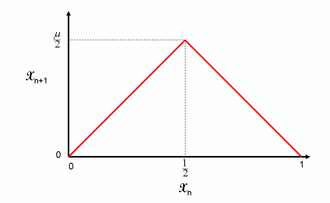
\includegraphics[width=0.5\linewidth]{Images/Tent Map.png}
        \caption{Tent Map}
    \end{figure}
\end{defn}
\begin{defn}
    Let $(X_i)$ be a sequence of continua such that for all $i\geq 1,$ 
    \[f_{i+1}: X_{i+1}\to X_i\] is a sequence of continuous surjective maps. Then we define 
    \[X_\infty := \lim_{\leftarrow}(X_i, f_i) = \{x_i \in \prod X_i \; ; \; x_i = f_{i+1}\; \forall i\}\] as the \textbf{inverse limit}, as a subset of $\prod X_i.$ 
\end{defn}
 \[ \cdots \xrightarrow{} X_3 \xrightarrow{f_3} X_2 \xrightarrow{f_2} X_1.\] 
 \begin{thm}
     $X_\infty$ is a continuum and if $A_\infty \subset X_\infty$ is a sub-continuum, then $A = \lim_{\leftarrow}(A_i, g_{i+1})$ where $A_i = \pi_i(A), g_{i+1} = f_{i+1} |_{A_{i+1}}$
 \end{thm}
 \begin{proof}
     Define 
     \[Q_{n,i} := \{(x_i) \in \prod X_i \; ; \; x_i = f_{i+1}(x_{i+1}), \; \forall i \in [n]\}.\] Since $Q_n \approx \prod_{i\geq n} X_i,$ then $Q_n$ is nonempty, compact, Hausdorff, and connected. -
 \end{proof}
 
\end{exmp}

\newpage
\subsection*{Tuesday, Feb 11: Regular and Normal results}
\begin{rem}
    \begin{enumerate}
        \item T0- Points are closed (a  point)
        \item T1-Hausdorff
        \item T2-Regular
        \item T3-Normal
    \end{enumerate}
\end{rem}
\begin{lemma}
    Suppose points are closed in $X.$ Then 
    \begin{enumerate}
        \item $X$ is regular if and only if for all $u\in X,$ for all open $U\ni u,$ there exists a $V\ni u$ open such that $\overline{V} \subset U$ 
        \item $X$ is normal if and only if for all $A\subset X$ closed, for all $U\supset A$ open, there exists a $V\supset A$ open such that $\overline{V}\subset U.$
    \end{enumerate}
\end{lemma}
\begin{proof}
    (a) If $X$ is regular, then there exists some open set $U$ containing $x.$ Thus, $X\setminus U$ is closed and disjoint from $\{x\}.$ By  regularity, there exists $V\ni u$ open such that $W \supset X\setminus U$ open and $V\cap W = \emptyset.$ We have that $V \supset X\setminus W,$ the latter of which is closed, and thus $\overline{V}\subset X\setminus W \subset U$

    Let $x\in X,$ and suppose $K\subset X$ is closed with $x\notin K.$ $X\setminus K = U$ is open and contains $x,$ and thus by assumption, there exists some $V\ni x$ such that $\overline{V} \subset U,$ and thus $X\setminus \overline{V}$ is open and contains $K$ and is disjoint from $V.$ 

    (b) Replace $x$ with $A$ above.
\end{proof}
\begin{thm}
    The following hold:
    \begin{enumerate}
        \item The subspace of a Hausdorff space is Hausdorff. Moreover, an arbitrary product of Hausdorff spaces is Hausdorff
        \item A subspace of a regular space is regular and an arbitrary product of regular spaces is regular.
    \end{enumerate}
\end{thm}
\begin{rem}
    The subspace of a normal space is not necessarily normal, and the product of normal spaces is not necessarily normal.
\end{rem}
\begin{proof}
    (b) Suppose $X$ is our regular space, and $Y\subset X$ is a subspace. Suppose $y\in X$ and $A\subset Y$ is closed and $\{x\}\cap A = \emptyset.$ Thus, $A = Y \cap K$ for some $K\subset X$ closed. So then $\{x\}\cap K = \emptyset,$ and so there exists $U\ni x$ and $V\supset K$ both open and disjoint. Then $Y\cap U$ and $Y\cap V$ are both open and disjoint, and we are done.

    Suppose $\{X_\alpha\}$ are all regular, then they are Hausdorff, and so $X = \prod X_\alpha$ are all Hausdorff, and so points are closed. Let $x = (x_\alpha)\in X.$ Then if $U\ni x$ open (where $U$ is a basis). Thus, for all $\alpha,$ $x_\alpha \in U_\alpha \subset X_\alpha,$ and there exists $x_\alpha \in V_\alpha \subset U_\alpha$ where $\overline{V_\alpha}\subset U_\alpha.$ Evidently, $V = \prod V_\alpha,$ and $V\ni x,$ and we claim that 
    \[\overline{V} = \overline{\prod V_\alpha} = \prod \overline{V_\alpha}\subset \prod U_\alpha = U\]
\end{proof}

\begin{thm}
    If $X$ is regular with a countable basis, then $X$ is normal.
\end{thm}
\begin{proof}
    Let $\cal B$ be a countable basis. Let $A,B$ be closed disjoint subsets of $X.$ For all $x\in A,$ $x\in X\setminus B$ open, and thus there exist $U_x\ni x$ such that $\overline{U_x}\subset X\setminus B.$ Without loss of generality, we can assume $U_x$ is a basis element. Since $\cal B$ is countable, we can find $W_1, W_2, \dots$ basis elements such that $\overline{W_i} \cap B = \emptyset$ for all $i,$ and $\bigcup W_i \supset A.$ Similarly for $B$, there exists $V_1, V_2, \dots$ such that $\overline{V_i} \cap A = \emptyset$ for all $i$ and $\bigcup V_i \supset B.$

    Let \[W_1' := W_1\setminus \overline{V_1} = W_1 \cap (\overline{V_1}^c), \quad V_1' = V_1 \cap (\overline{W_1}^c),\] and note both are open and $A\cap W_1 = A\cap W_1'$ and similarly for $V_1'$. Define
    \[W_2' = W_2 \cap \overline{V_1}^c \cap \overline{V_2}^c, \quad V_2' = V_2 \cap \overline{W_1}^c \cap \overline{W_2}^c\] Build this recursively. The for any $n,$ $W_n'$ is disjoint from $V_j'$ with $j\leq n$ and $V_n'$ is disjoint from $W_j'$ with $j\leq n.$ Define 
    \[W:= \bigcup W_i'\supset A, \qquad V:= \bigcup V_i'\supset B\] open and disjoint.
\end{proof}

\begin{thm}
    Every metric space is normal.
\end{thm}
\begin{proof}
    Suppose $X$ is a metric space induced by the topology and let $A, B$ be disjoint closed sets. For all $a\in A,$ ther exists an $\epsilon_a >0$ such that 
    \[B_{\epsilon_a}(a) \cap B  = \emptyset, \qquad B_{\epsilon_b}(b) \cap A  = \emptyset\]
    Let \[U := \bigcup_{a\in A} B_{\frac{\epsilon_a}{2}}(a), \quad V := \bigcup_{b\in B} B_{\frac{\epsilon_b}{2}}(b)\] Both are open. Suppose $x\in U \cap V,$ then $v\in B_{\frac{\epsilon_a}{2}}(a) \cap B_{\frac{\epsilon_b}{2}}(b),$ for some $a\in A,$ $b\in B,$ and thus 
    \[d(a,b)\leq d(a,x) + d(x,b) < \epsilon = \min\{\epsilon_a, \epsilon_b\} \implies b \in B_{\epsilon_a}(a).\]
\end{proof}

\begin{thm}
    Compact Hausdorff spaces are normal. 
\end{thm}
\begin{proof}
    Let $A,B$ be closed disjoint sets. For all $a\in A,$ there exists $U_a\ni a$ and $V_a \supset B$ open and disjoint. 
    \[A \subset \bigcup_{a\in A} U_a \implies A\subset \bigcup_{i=1}^N U_{a_i} =:U.\] Moreover, 
    \[V:=\bigcap_{i=1}^N V_{a_i}\supset B.\] $U$ and $V$ are open disjoint. 
\end{proof}
\begin{rem}
    To recap:
    For compact $X,$ the following are equivalent:
    \begin{enumerate}
        \item $X$ is regular
        \item $X$ is Hausdorff
        \item $X$ is normal
    \end{enumerate}
    For second countable $X$:
    \begin{enumerate}
        \item $X$ is regular
        \item $X$ is normal
        \item $X$ is metrizable.
    \end{enumerate}
    Thus, we have yet to prove the last equivalence.
\end{rem}
\begin{lemma}
    (Urysohn's Lemma) Let $X$ be normal, $A, B \subset X$ be closed and disjoint. Then there exists a continuous function $f: X\to [0,1]$ such that $f(A) = 0$ and $f(B) = 1.$
\end{lemma}
\begin{proof}
    Let $P = \bbQ \cap [0,1].$ For each $p \in P,$ we want to find some $U_p$ open such that $A\subset U_0,$ $U_1 = X\setminus B,$ and if $p < q,$ then $\overline{U_p}\subset U_q.$

    Let $U_1 = X\setminus B$ and since $A\subset U_1,$ then by normality, there exists some $A\subset U_0$ such that $\overline{U_0}\subst U_1.$ By normality, there exists some open $\overline{U_0}\subset U_\frac{1}{2}$ such that $\overline{U_\frac{1}{2}}\subset U_1.$ Keep going with the fairy rationals. Let $U_\frac{p}{q} = X$ if $\frac{p}{q} >1,$ and Define 
    \[f(x): = \inf\{\frac{p}{q}\text{ such that } x\in U_\frac{p}{q}\}.\] We claim that $f$ is our function.
\end{proof}

\newpage
\subsection{Tuesday, Feb 18:}

\begin{thm}
    Suppose $X$ is regular with a countable basis. Then $X$ is metrizable.
\end{thm}
\begin{proof}
    We use Urysohn's Lemma. For all $x\in X,$ for all $U$ open, there exists $f: X\to [0,1]$ continuous such that $f(x) = 1$ and $f(X^c) = 0.$

    We claim that if $X$ is completely regular, then there exists an embedding from $X\mapsto [0,1]^J,$ for some $J$ index set In fact, $X$ completely regular and a countable basis implies there exist an embedding from $X\mapsto [0,1]^N.$ It suffices to show this, since $X$ would be homeomorphic to a subset of a metric space.

    \begin{enumerate}
        \item If $X$ is compltely regular the for all $x\in X,$ for all $U \ni x$ open, then we choose $f: X \to [0,1]$ with $f(x) = 1$ and $f(X^c) = 0.$ We take these $f$ to be the coordinates of 
        \[F: X \to [0,1]^J.\] If $x\neq y,$ then we can choose $x\in U$ and $y\notin U$ such that $f(x) = 1$ and $f(y)  = 0,$ and so the map is injective. $F$ is continuous and injective, to show that $F$ is a homeomorphism unto its image, we want to show that $F^{-1}: F(X) \to X$ is continuous. That is, for all $U \subset X$ is open, then $F(U)\subset F(X)$ is open. That is, we want to show that $F(U) = F(X) \cap V,$ $V\subset [0,1]^N$ is open. Let $F(x) \in F(U)$ for some $x\in U.$ We want to find some open $W = F(X) \cap V$ such that  $F(x) \in W.$ Let \[V := \pi_f^{-1}((0,1]) \subset \prod_J [0,1],\] which is obviously open, then $F(x)\in V\cap F(X)\subset F(U)$
        \item If $F$ has a countable basis, then we claim that we can find a countable set $f_n: X\to [0,1]$ continuous such that for all $x\in X,$ for all $U\ni x,$ open, there exists some $n$ such that $f_n(x) = 1$ and $f_n(X^c) = 0.$ Let $\{U_i\}$ be a countable basis, and suppose $x\in U$ open. Then $x\in U_i \subset U,$ then since $X$ is regular, $x \in \overline{U_j}\subset U_i \subset U.$ Define $f_{i,j}: X\to [0,1]$ such that $f_{i,j}(\overline{U_j}) = 1$ and $f_{i,j}(U_i^c) = 0.$
        \item Take $f_{i,j}$ from above as the coordinates of $F,$ and so $F: X\to [0,1]^N$ is a homeomorphism unto its image. Thus, $X$ is metrizable.  
    \end{enumerate}
\end{proof}

\begin{prop}
    Let $\overline{X} = \overline{F(X)}\subset [0,1]^J.$
    \begin{enumerate}
        \item $\overline{X}$ is compact and Hausdorff.
        \item If $X\subset \overline{X}$ is dense and $X$ has subspace topology.
        \item For all $f: X\to [0,1],$ there exists a unique $\overline{f}: \overline{X}\to [0,1].$
    \end{enumerate}
\end{prop}
\begin{lemma}
    Suppose $\overline{X}$ is compact and Hausdorff. Then $\overline{f}: \overline{X}\to [0,1]$ and $\overline{f}|_X = f,$ then $\overline{f}$ is defined by $f.$ That is, the extension is unique.
\end{lemma}

\begin{thm} (Stone-\^{C}ech compactication)
    Let \( X \) be a completely regular space. There exists a compact Hausdorff space \( \beta X \) and a homeomorphism mapping \( X \) into a dense subset of \( \beta X \) such that if \( f \) is a bounded continuous function from \( X \) to \( \mathbb{R} \), then \( f \) has a bounded continuous extension to \( \beta X \).
\end{thm}

\begin{thm}
    (Alexandroff- Hausdorff) Let $X$ be Hausdorff, the following are equivalent:
    \begin{enumerate}
        \item There is a continuous surjective map $f: C\to X$
        \item $X$ is nonempty, compact, and metrizable.
        \item $X$ is nonempty, compact, and has a countable basis.
    \end{enumerate}
\end{thm}
\begin{rem}
    For a compact Hausdorff $X,$ metrizable is equivalent to $X$ having a countable basis from before.
\end{rem}

\begin{lemma}
    Suppose $f: A\to B$ is continuous and surjective. If $A$ is compact and metrizable, and $B$ is Hausdorff, then $B$ is compact and metrizable.
\end{lemma}
\begin{proof}
    It suffices to show that $B$ has a countable basis. Let $\cal U_n$ be a countable basis for $A.$ Let $\cal U'_k$ be another countable basis for $A$ such that each $U_i' = \displaystyle\bigcup_{j=1}^N U_j.$ Define 
    \[V_i := B - f(A - U_i').\] We claim that $\{V_i\}$ is a basis for $B.$ $V_i$ is obviously open. Let $b\in B.$ Let $b\in V\subset B$ be open. It suffices to find some $V_i \in \{V_i\}$ such that $b\in V_i \subset V \subset B.$ $f^{-1}(\{b\})$ is compact and contained in $f^{-1}(V)$ open. For all $a\in f^{-1}(\{b\}),$ $a\in U_j$ for $U_j \subset f^{-1}(V).$ By compactness, there exist finitely many of these, $U_i$ so take the union to make $U_i'$ and thus 
    \[f^{-1}(\{b\}) \subset U_i' \subset f^{-1}(V)\implies A - f^{-1}(\{b\}) \supset A - U_i' \supset A - f^{-1}(V) \implies f(A - f^{-1}(\{b\})) \supset f(A - U_i') \supset f(A - f^{-1}(V))\] and so 
    \[ B - f(A - f^{-1}(\{b\})) \subset B - f(A - U_i') \subset B - f(A - f^{-1}(V))\] and it can be shown that this is equivalent to
    \[\{b\} \subset V_i \subset V\]
\end{proof}
\begin{proof} (Alexandroff-Hausdorff)
    Suppose $f: X\to X$ is continuous and surjective, then clearly, $X$ is nonempty and $X$ is compact. We claim that $X$ has a countable basis, which is obvious from our lemma.
\end{proof}

\begin{defn}
    Suppose $X$ is Hausdorff. Let $x\in X.$ The \textbf{connected component} of $X$ containing $x$ is the \textbf{maximal connected} subset of $X$ containing $x.$ 
\end{defn}
\begin{rem}
    This is equivalent to saying that 
    \[\text{component} = \bigcup Q \quad \text{st } Q\subset X \text{ is connected}\]
\end{rem}

\begin{defn}
    $X$ is totally disconnected if every connected component is a single point.
\end{defn}

\begin{defn}
    $X$ is \textbf{perfect} if no point is open.
\end{defn}
\begin{rem}
    $X$ is perfect if for all $x\in X,$ for all $U\ni u$ open, there exists $y\in U - x.$ That is, there are no isolated points.
\end{rem}

\begin{prop}
    Suppose $X = \displaystyle\prod_{i=1}^\infty X_i,$ where each $X_i$ is finite, nonempty, and is equipped with the discrete topology. Then $X$ is compact, nonempty, metrizable, and totally disconnected. Moreover, if infinitely many $X_i$ have more than $1$ point, then $X$ is perfect
\end{prop}
\begin{proof}
    Compact comes from Tychonoff. $X$ is metrizable from before. $X$ is obviously nonempty. To show that $X$ is totally disconnected
    
\end{proof}

\newpage
\subsection*{Feb 25: }


\end{document}